% 2.  Tecnologie di riferimento
% 2.1  Programmazione agile  (standup mattutino, usavamo trello) usato solo internamente perchè al cliente è stato venduto come progetto 
%infrastructure-as-a-code -> cloud formation 
% 2.2  Infrastrutture cloud  (caratteristiche in particolare di quella considerata)
% 2.2.1  Architetture serverless
% 2.3  Piattaforme Big Data  (caratteristiche e requisiti) chiedere?
% dare il contesto della data platform (spiegare cos'è, che si basa su una lambda architecture, il tool è tuttavia agnostico rispetto a alla piattaforma)
% 2.4  Strumenti utilizzati  (es. React, container e microservizi, , nodejs, k8s ...)
% In questo capitolo non deve scrivere tutto lo scibile riguardo a questi argomenti, ma solo quanto serve per far capire cosa lei ha fatto, dando riferimenti bibliografici per ciò che non è rilevante ai fini del suo lavoro.
\graphicspath{{./chapters/images/}}
\newtheorem*{definition}{Definition}

\chapter{Reference Technologies}
% Several tools, both technological and organizational, were required for this job.
The platform chosen to host the new web application is Amazon Web Services \cite{aws}. The choice was forced by the fact that the customer data platform was already in place and the application is closely tied to that environment. Before diving into the details of the project, let us see an overview of the reference technologies that power AWS.

% \section{AGILE Software Development}
% not worth it for just the standups



\section{Cloud Infrastructure}
Cloud Infrastructure is a term used to describe the set of components, like hardware, abstracted resources, storage and network resources needed for cloud computing; think of it like the tools needed to build a cloud.
Let us start with a definition of Cloud Computing:

\begin{definition}
  Cloud computing is a remote, virtual pool of on-demand, shared resources that can be rapidly deployed at scale.\cite{cloud}
\end{definition}

The basic concept to understand from this definition is the \emph{virtualization}: this is an abstraction technology, used to separate resources from physical hardware and pool them into clouds; in essence, it allows you to create multiple virtual machines, all of which run on a single server. Each one has its own operating system and set of applications, and can run all at the same time without being aware of each other's existence.

With virtualization, an organization can reduce its Capital Expenditure (CapEx), namely the funds used to acquire, upgrade and maintain the physical hardware of on-premise servers, and thus reduce its Operational Expenditure (OpEx), as it would not need to rent a facility to house them or pay salaries for any maintainer because all the costs involving the hardware are borne by the cloud provider. 

There are 4 main types of resources that can be built with these virtual machines:
\begin{itemize}
    \item Compute resources provide on-demand processing power to complete a workload; these are used to run programs or scripts in the cloud. An equivalent in the traditional on-premise environment would be the physicals servers that you would connect to remotely, install, and run software on.
    \item Storage resources allow to save and retrieve unstructured data; these are resources that allow you to store things like images or videos in the Cloud. Here the equivalent would be a DAS (direct attached storage), NAS (Network attached storage), or SAN (storage area network).
    \item Database resources allow to store structured sets of data to be used in an application.
    \item Network resources allow to control how all the other resources will communicate with each other. In a data center, this role would be taken by routers, switches, firewalls, and load balancers.
\end{itemize}

\subsection{Cloud Service Models}
A Cloud Vendor offers different type of services to the customers, where "as-a-Service" generally means a cloud computing service that is managed in lieu of the customer.
\begin{figure}[!htb]
    \centering
    \includesvg[inkscapelatex=false, width = 15.8cm]{ch_2/cloud/saas-paas-iaas-diagram}
    \caption{The elements included with each type of service. \cite{model}}
    \label{fig:cloud_service_models}
\end{figure}

\subsubsection{Infrastructure-as-a-Service (IaaS)}
This is the most basic model where the cloud provider hosts the infrastructure, providing virtualization, storage, servers, wires and appliances that make connections between those machines, on behalf of their customers, essentially taking care of the hardware, so that the user does not have to have an on-premise data-center and does not have to worry about physically updating and maintaining those components; however, it is the responsibility of the customer to handle the applications, data, operating system, middle-ware, and runtimes. 

As shown in Figure \ref{fig:iaas}, the user can access the infrastructure via any Internet connection as opposed to on-premise solution, where the user has to physically be in the data-center.

\begin{figure}[!htb]
    \centering
    \includesvg[inkscapelatex=false, height=6cm, width = 15.8cm]{ch_2/cloud/iaas}
    \caption{On-Premise vs. IaaS. \cite{iaas}}
    \label{fig:iaas}
\end{figure}


\subsubsection{Platform-as-a-Service (PaaS)}
The cloud provider hosts the hardware and provides an application software platform, such as the operating system. It is primarily intended for developers and programmers as it allows them to develop, run, and manage their own apps without having to build and maintain the infrastructure or the platform. PaaS can be accessed over any Internet connection, making it possible to build an entire application in a web browser. 

Among the tools provided with PaaS are: 
\begin{itemize}
    \item a set of development tools, sometimes offered together as a framework, including, a source code editor, a debugger, a compiler, and other essential tools. 
    \item Middleware that sits in between user-facing applications and the machine's operating system, which is necessary for running the application, but end users do not interact with it.
    \item Operating Systems where the developers work on and the application run on.
    \item Databases administered and maintained by the vendor, which usually provides developers with a database management system.
\end{itemize}

This service is often used by developers for a number of reasons, like the ability to cut coding time by leveraging pre-coded application components built into the platform, the support for geographically distributed teams because the development environment is accessed over the Internet, and the efficient management of the application life-cycle by building, testing, deploying, managing, and updating within the same integrated environment.


\subsubsection{Software-as-a-Service (SaaS)}

This service is a form of cloud computing where users subscribe to an application rather than purchasing it once and installing it. Figure \ref{fig:saas} shows that the actual application logic runs in the cloud and many users can log into it and use it from any compatible device. The SaaS model reduces the users' upfront costs by eliminating the need to permanently purchase software, however they should invest in fast network hardware since service performance is determined by Internet connection speeds.

\begin{figure}[!htb]
    \centering
    \includesvg[inkscapelatex=false, width = 7.9cm]{ch_2/cloud/saas1}
    \includesvg[inkscapelatex=false, width = 7.9cm]{ch_2/cloud/saas2}
    \caption{Where the application logic lies. \cite{saas}}
    \label{fig:saas}
\end{figure}

\subsection{Private, Public, and Hybrid}
If the models above defined how the services are offered via the cloud, then these different cloud deployment models define where the cloud server are and who manages them.

\subsubsection{Private Cloud}
A private cloud is a server, data-center, or distributed network entirely dedicated to one organization. By using a private cloud, an organization can experience the benefits of cloud computing without sharing resources with other organizations. As shown in Figure \ref{fig:private_internal_or_hosted}, this type of cloud can either be located inside an organization (on-premise) or remotely managed by a third party and accessed over the Internet (off-premise). It should be noted that an internal private cloud is not the same as a traditional data-center, because, as a cloud model, it boasts all the features of the cloud architecture, like virtualization, which makes them more efficient, more powerful, and more scalable.


\begin{figure}[!htb]
    \centering
    \includesvg[inkscapelatex=false, width = 15.8cm]{ch_2/cloud/private-cloud-internal-vs-hosted}
    \caption{Different locations for the private cloud. \cite{private}}
    \label{fig:private_internal_or_hosted}
\end{figure}

A reason to use the private cloud model may depend on a company's security standard because it eliminates inter-company \emph{multi-tenancy}, which is when multiple customers of a cloud provider are accessing the resources provided by the same physical server, like data or processes. This gives a company more control over the cloud security measures that are put in place, despite the increase in cost that this approach will need.

\subsubsection{Public Cloud}
A public cloud is a pool of virtual resources that is automatically provisioned and allocated among multiple clients through a self-service interface.

\begin{figure}[!htb]
    \centering
    \includesvg[inkscapelatex=false, width = 15.8cm]{ch_2/cloud/public-cloud-vs-private-cloud}
    \caption{Distinct utilization for private and public cloud models. \cite{public}}
    \label{fig:private_vs_public}
\end{figure}

The distinction from private cloud model, highlighted in Figure \ref{fig:private_vs_public}, relies on the fact that the private model is a cloud service that is not shared with any other organization, which avoids multi-tenancy and increases data protection; by contrast, a public cloud is a cloud service that shares computing services among different customers, while protecting and hiding each customer's data and applications from one another.

\pagebreak

\subsubsection{Hybrid Cloud}
A hybrid cloud mixes two or more types of cloud environments, which combines public and private cloud, both on-premise and hosted. These different cloud environments must be tightly interconnected with each other, essentially functioning as one combined infrastructure.

\begin{figure}[!htb]
    \centering
    \includesvg[inkscapelatex=false, width = 15.8cm]{ch_2/cloud/hybrid_cloud}
    \caption{Each cloud environment is presented as one to the client. \cite{hybrid}}
    \label{fig:hybrid}
\end{figure}

\subsection{Microservice Architecture}
Before cloud and cloud computing came to be, the classic way to build an application was with a Monolithic Architecture, usually hosted on a specific server or set of servers, which consist of a single stack: the User Interface on top, the Business Logic in the middle, and the database on the bottom.
Such architecture has several disadvantages; for example, any change, does not matter how minimal, means the entire stack has to be updated, or if a portion of the application breaks, the entire application might fail.

With the cloud, the idea came forth of dividing a larger application in smaller, independent services, thus a Microservice Architecture was born. A microservice is a smaller portion of an application, that performs one service only, runs in its own environment independently from other parts of the application, and accesses its own data. Figure \ref{fig:monolithic_vs_microservice} shows a comparison between the two approaches; we can see that a user will not be able to distinguish between them.

\begin{figure}[!htb]
    \centering
    \includesvg[inkscapelatex=false, width = 15.8cm]{ch_2/cloud/monolithic-architecture-vs-microservices-architecture}
    \caption{Side-by-side comparison between the architectures. \cite{micro}}
    \label{fig:monolithic_vs_microservice}
\end{figure}

This kind of architecture has several advantages:
\begin{itemize}
    \item Resilience: as the services are independent from one another, the breaking or crashing of a service does not affect the rest of the application.
    \item Selective scalability: instead of scaling the entire application, only the service that receive a large amount of usage can be scaled.
    \item Easier to handle change: new features or updates can be rolled out one at a time, instead of re-deploying the entire application stack.
    \item Flexibility for developers: each service is independent, and as such could be written in different languages. 
\end{itemize}

The main advantage of building an application with a Microservice Architecture in the cloud is most evident when used in conjunction with a Serverless architecture which allows a service, or even a function, to be executed only when needed.

\subsection{Serverless Architecture}
\begin{definition}
Serverless computing is a method of providing back-end services on an as-used basis.\cite{sls}
\end{definition}

From this definition of Serverless, we can infer that the resources needed to provide computing power for a back-end infrastructure are not reserved and paid for upfront, instead they are provided on-demand and charged based on usage. There are still servers in serverless, but they are abstracted away from the application development.

The Serverless provider manages all the underlying infrastructure, allowing the users to only worry about code development and deployment, while ensuring auto-scaling of the service in case of peak activity. The Figure \ref{fig:serverless_benefits} shows the difference in costs between a classic cloud approach and a Serverless one. With traditional servers, developers and companies purchase a fixed number of servers, or an amount of server space, to ensure that a spike in traffic or activity does not exceed their monthly limits, thus breaking the application; this would mean that part of the purchase could be wasted. On the other hand, with the Serverless approach they can purchase back-end services on a pay-as-you-go basis.



\begin{figure}[!htb]
    \centering
    \includesvg[inkscapelatex=false, width = 15.8cm]{ch_2/cloud/benefits-of-serverless}
    \caption{A representation of the benefits of Serverless. \cite{sls}}
    \label{fig:serverless_benefits}
\end{figure}



\subsection{Function-as-a-Service} \label{FaaS}
Function-as-a-Service (FaaS), or Serverless computing, is an event-driven execution model that runs in stateless containers that allow developers to build, compute, run, and manage application packages as functions without having to maintain their own infrastructure. This is a serverless way to implement a microservice architecture, and since this functions are stateless, they are inherently scalable.

Figure \ref{fig:monolithic_breakdown} shows the breakdown of a monolithic application in distinct microservices, which in turn are divided in functions where each is an implementation of FaaS. 
\begin{figure}[!htb]
    \centering
    \includesvg[inkscapelatex=false, width = 15.8cm]{ch_2/cloud/monolithic-application-microservice-faas}
    \caption{Breakdown of a monolithic application into simple functions. \cite{faas}}
    \label{fig:monolithic_breakdown}
\end{figure}

We can see that, by using FaaS as building blocks of microservices, we can build a truly modular application.

\subsubsection{PaaS vs. Serverless computing}

PaaS and Serverless computing are similar in that for both a developer has to worry only about writing and uploading code, while the vendor handles all the back-end processes. However, there are key points of difference:
\begin{itemize}
    \item Scaling is vastly different when using the two models since applications built using Serverless computing, or FaaS, will scale automatically, whereas PaaS applications will not unless programmed to do so. 
    \item While PaaS applications are more like traditional applications, and have to be running most of the time or all of it in order to be immediately available for users, Serverless applications can be up and running almost instantly.
    \item With Serverless computing vendors do not provide development tools or frameworks, while they do with PaaS.
    \item PaaS billing is not nearly as precise as in Serverless computing, in which charges are broken down to the number of seconds or fractions of a second each instance of a function runs.
\end{itemize}


\section{Amazon Web Services}
This section will outline the key AWS services used in the project.

\subsection*{AWS API Gateway}
In general, an API gateway is an API management tool that sits between a client and a collection of back-end services, and acts as a reverse proxy to accept all API calls, aggregate the various services required to fulfill them, and return the appropriate result.
% \begin{wrapfigure}{r}{0.25\textwidth} %this figure will be on the right
%     \centering
%     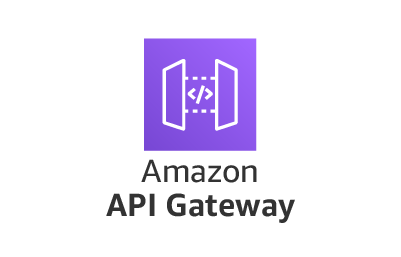
\includegraphics[width=3.5cm]{chapters/images/ch_2/AWS/AWS_APIGW.png}
% \end{wrapfigure}


Amazon API Gateway \cite{apigw} is a service for building comprehensive RESTful API that are HTTP-based, that enable stateless client-server communication, and implement standard HTTP Create, Read, Update, and Delete methods.

\begin{figure}[!htb]
    \centering
    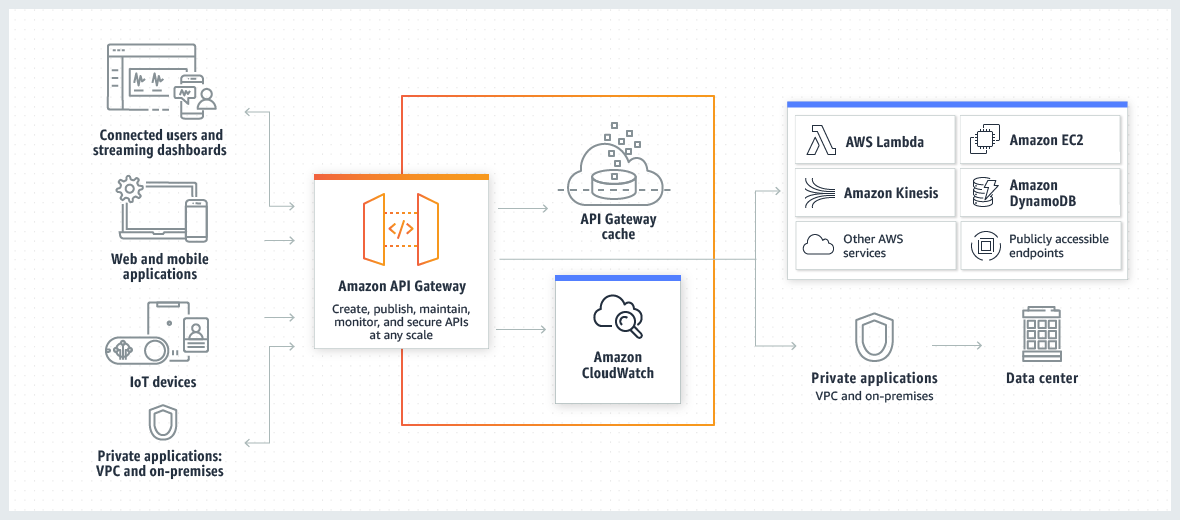
\includegraphics[ width = 15.8cm]{chapters/images/ch_2/AWS/AWS_APIGW_diagram.png}
    \caption{API Gateway diagram. \cite{apigw}}
    \label{fig:AWS_APIGW_diagram}
\end{figure}

The diagram in Figure \ref{fig:AWS_APIGW_diagram} illustrates how the API Gateway provides a developer with an integrated and consistent development experience for building AWS Serverless applications. API Gateway handles all the tasks involved in accepting and processing up to hundreds of thousands of concurrent API calls, essentially acting as a ``front door'' for applications to access data, business logic, or functionalities from the back-end services.

\subsection*{AWS Lambda}
AWS Lambda \cite{lambda} is an implementation of FaaS, or Serverless computing. As mentioned in \ref{FaaS}, code can run for virtually any type of application or back-end service, and the Lambda takes care of everything required to run it and scale it with high availability. 



\subsection*{Amazon Aurora}
Amazon Aurora \cite{aurora} is a relational database engine that combines the speed and reliability of high-end commercial databases with the simplicity and cost-effectiveness of open source databases. As shown in Figure \ref{fig:AuroraArch}, it is designed to replicate 6 copies of the data across 3 different Availability Zones, thus creating a distributed, fault-tolerant, and self-healing storage system.  

\begin{figure}[!htb]
    \centering
    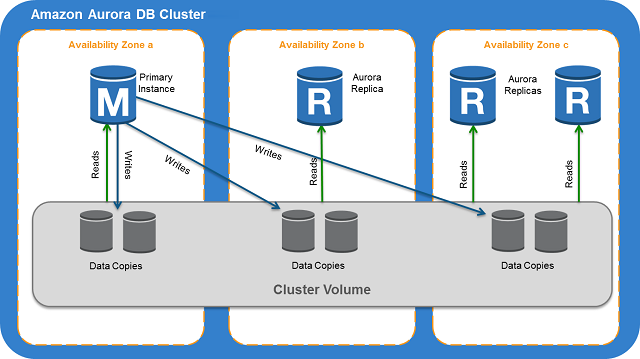
\includegraphics[ width = 15.8cm]{chapters/images/ch_2/AWS/AuroraArch.png}
    \caption{Aurora data replication schema. \cite{auroraSchema}}
    \label{fig:AuroraArch}
\end{figure}

\subsection*{Amazon Simple Queue Service}
SQS \cite{sqs} is a managed queuing service that enables the secure message exchange, decoupling and scaling of microservices and serverless applications from one another. With it, it was possible to perform the logging of the operations performed and the asynchronous invocation of actions, while also providing a near real-time experience for the users.

\subsection*{Amazon Elastic Container Registry}
Amazon ECR \cite{ecr} is a managed container registry used by developers to share and deploy container images, keep track of the created versions, and manage their lifecycle. Moreover, these images are transferred to the registry via the HTTPS protocol and are encrypted at rest. 

\begin{figure}[!htb]
    \centering
    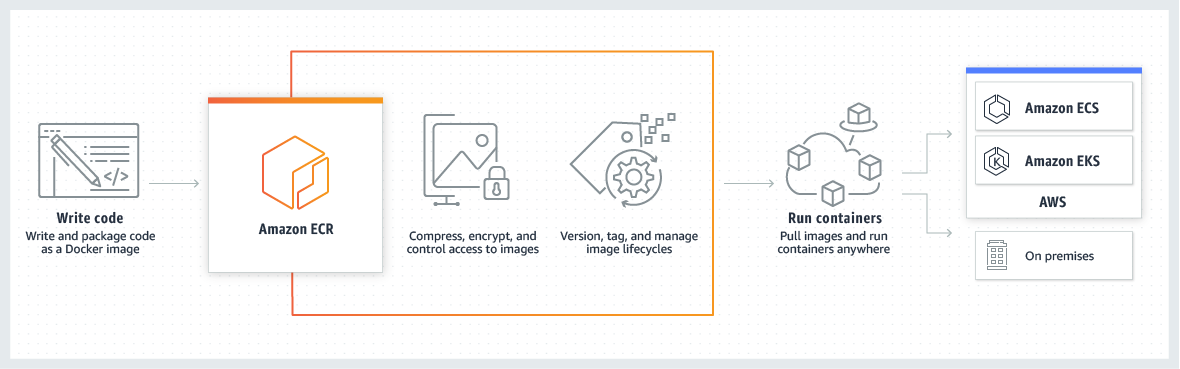
\includegraphics[ width = 15.8cm]{chapters/images/ch_2/AWS/ecr.png}
    \caption{ECR diagram. \cite{ecr}}
    \label{fig:AWS_ecr}
\end{figure} 

\subsection*{Amazon CloudFormation}
CloudFormation \cite{cloudFormation} is a service that uses template files to automate the configuration of AWS resources. As further defined in \ref{IaC}, it can be described as an Infrastructure-as-Code tool and a Cloud Automation solution, which is the use of automated tools and processes to perform workflows in a cloud environment that would otherwise have to be performed manually, such as configuring servers or setting up a network, thereby enabling the automated setup and deployment of virtually any AWS service.  

\begin{figure}[!htb]
    \centering
    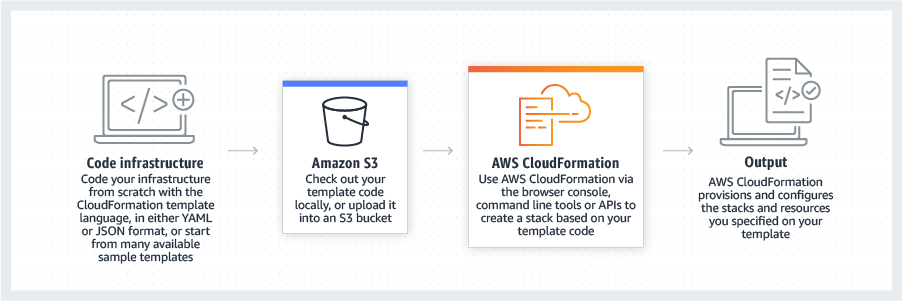
\includegraphics[ width = 15.8cm]{chapters/images/ch_2/AWS/AWS_cloudFormation.png}
    \caption{CloudFormation deployment process. \cite{cloudFormation}}
    \label{fig:cloudFormation}
\end{figure}

\section{Big Data Platform}
In the process of Digital Transformation of the customer, aimed at digitizing processes and enabling new business models, we find the Integrated Data Platform, whose goal is to make the most of the data produced every day by the company and turn them in valuable elements for the business. It is the cornerstone of the business' data strategy that ensures centralized information governance and enables coexistence and inter-operability of on-premise hosted, private and public cloud data resources.

The main benefits of the Data Platform will be:
\begin{itemize}
    \item Data-driven approach that will support the decision making process.
    \item Smart Manufacturing that will allow factories to monitor, analyze, and improve production.
    \item A centralized, integrated location that helps information cross between central systems and factories.
    \item Predictive Analysis applicable to both production facilities and new types of products enabling the creation of new business models.
    \item The Data Lake, with its large amount of data, computing power and services offered by the Cloud Provider enable the use of AI/ML.
\end{itemize}

The Data Platform is designed to support the numbers shown in Figure \ref{fig:DP_amount} in terms of integrated data and their processing:
\begin{figure}[!htb]
    \centering
    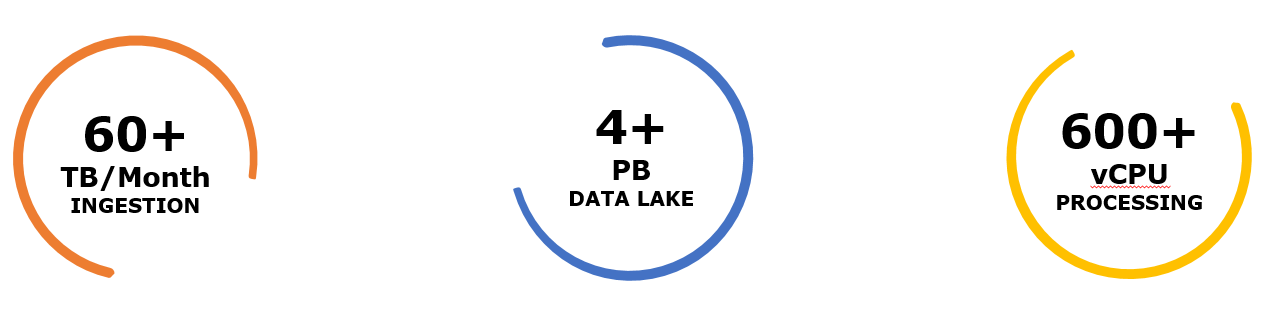
\includegraphics[ width = 15.8cm]{chapters/images/ch_2/DP_amount.png}
    \caption{Amount of data and processing power of the Data Platform.}
    \label{fig:DP_amount}
\end{figure}
\begin{itemize}
    \item The platform handles the loading of more than 60 TB/Month composed of both Near Real Time and event-driven Batch streams.
    \item Since the Data Platform must retain a 5-year history and based on the amount of data produced each day, it is estimated to have a Data Lake with a size rater than 4 PB.
    \item To support data loading, transformation, consolidation, and visualization, we are provided with a high computing power of more than 600 vCPUs.
    
\end{itemize}

\section{ToolBox}
Several development tools were required for this project in addition to the cloud infrastructure. This section will give a brief introduction of each tool.

\subsection{Node.js }
Among the supported languages for AWS Lambda there is also Node.js \cite{node}, an open-source, cross-platform, back-end JavaScript runtime environment that runs on Chrome’s V8 engine and executes JavaScript code outside of a web browser.

\begin{definition}
Node.js is a JavaScript runtime built on Chrome’s V8 JavaScript engine. Node.js uses an event-driven, non-blocking I/O model that makes it lightweight and efficient. \cite{stein_2016}
\end{definition}

It is designed to build scalable network applications by leveraging its single-threaded and asynchronous event-driven runtime. A Node.js application runs in a single process, without creating a new thread for each request; when it performs an I/O operation, instead of locking the thread and wasting CPU cycles waiting, Node.js will make use of a thread taken from a thread pool to perform the task and will resume the operations when the response comes back. This allows Node.js to handle thousands of concurrent connections with a single server without the burden of handling thread concurrency, which could be a significant source of bugs. This is possible thanks to the Event Loop, depicted in Figure \ref{fig:EventLoop}.

\begin{figure}[!htb]
    \centering
    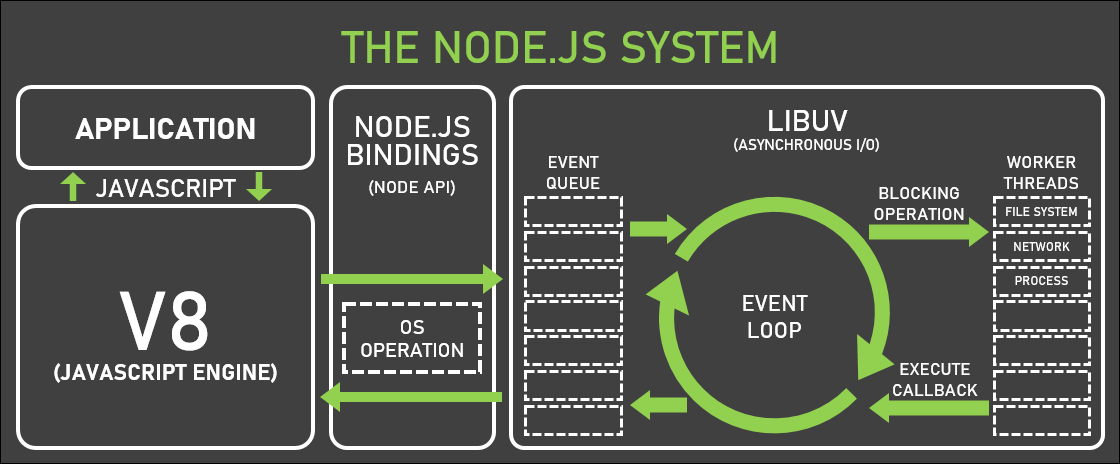
\includegraphics[ width = 15.8cm]{chapters/images/ch_2/Tools/Node.js-Event-Loop.png}
    \caption{Event Loop that powers Node.js. \cite{loop}}
    \label{fig:EventLoop}
\end{figure}

\subsubsection{TypeScript}
The language used for back-end and front-end development is TypeScript \cite{ts}, which is an object-oriented super-set of JavaScript that was developed to overcome code complexity for large projects. 

Javascript is a dynamically typed language, meaning that the software will not treat type differences as errors until runtime, which often results in bugs. TypeScript on the other hand offers optional static typing. Once static typing is declared, a variable does not change its type, and during compilation, the compiler alerts developers to any type of errors (syntactic or semantic), which results in early bug detection.



\subsection{Infrastructure as Code} \label{IaC}
Infrastructure provisioning has historically been a time-consuming and expensive manual process, completed by accessing a management portal and using a point-and-click approach to deploying resources.
Infrastructure as Code (IaC) is the managing and provisioning of infrastructure through code instead of manual processes. With this approach, configuration files that contain the infrastructure specifications are created, thus ensuring that the same environment is provisioned every time. By deploying the infrastructure as code also means that it is possible to divide it into modular components that can be automatically combined in different ways, and since it is provisioned via code, the configuration can be added to the version control system. 

The ultimate goal of IaC is automation as it is possible to integrate the process of provisioning, or dismantling, resources in any DevOps flow.

\subsubsection{Serverless Framework}
To this end, the Serverless Framework \cite{slsf} was used, which uses a command-line tool and configuration files to deploy both code and cloud infrastructure leveraging Cloud Formation templates, while also managing the lifecycle of the serverless architecture.


\subsection{OpenAPI Specification}
\begin{definition}
The OpenAPI Specification defines a standard, language-agnostic interface to RESTful APIs which allows both humans and computers to discover and understand the capabilities of the service without access to source code, documentation, or through network traffic inspection. \cite{openApi}
\end{definition}
With it, the API for each Lambda function was defined describing its path, HTTP method, possible path or query parameters, an authorizer to check user permissions to access a resource, validation of the request body, and the body of the response to the API call.


\subsection{Flyway} %database automation?
Flyway \cite{flyway} is an open-source database migration tool, and as such it allows you to transfer data from one type of database to another. However, we did not use it for data migration in the strict sense, but rather as a tool that allowed us to add changes to the database schema to the versioning system. 
With this tool, it is not necessary to interact directly with the Aurora instance to update the schema. At the time of migration, Flyway would check the back-log saved in the database itself, comparing the result of previous migrations with the current state of the schema.

To use Flyway's migration capability, migration files must be written in SQL and use the following naming convention:
\begin{figure}[!htb]
    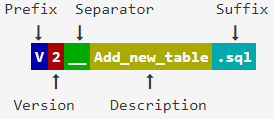
\includegraphics[ width = 7.5cm]{chapters/images/ch_2/Tools/flyway1.png} 
    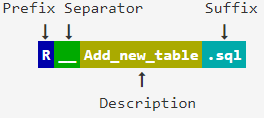
\includegraphics[ width = 7.5cm]{chapters/images/ch_2/Tools/flyway2.png}
    \caption{Naming convention for, respectively, versioned and repeatable migrations. \cite{migrate}}
    \label{fig:flyway}
\end{figure}
\begin{itemize}
    \item A prefix that represents the type of migration.
        \begin{itemize}
            \item \textbf{V} for versioned and \textbf{R} for repeatable. 
        \end{itemize}
    \item in case of a versioned migration, a version number to distinguish one version from another; the use of semantic versioning can help to keep track of the change introduced.
    \item Two underscores as separator.
    \item A description of the introduced change.
    \item The file suffix.
\end{itemize}

The versioned migrations are applied in order exactly once and each version migration has a unique version, a description, and a checksum that is used to detect accidental changes to an already applied version. In the project, this kind of migration has been used to keep record of the schema changes.

Repeatable migrations are applied after all pending versioned migrations have been executed and in the order of their description. Like the versioned migrations, they have a description and a checksum, but no version; moreover, they are applied whenever their checksum changes. In the project, they are used for the creation of views.

\subsection{React}
React \cite{react} is a declarative, efficient, and flexible JavaScript library for building interactive user interfaces. It lets you compose complex UIs from small and isolated pieces of code called \textit{components}. We used it with the AntDesign Pro framework to build the front-end side of the application.

\subsubsection{AntDesign Pro}
AntDesign Pro \cite{ant} is an open source code for enterprise-level UI design languages and React UI library. It comes with a set of high-quality React components, with theme customization capability.


\subsection{DevOps}

As a DevOps platform we used GitLab to host the GIT repository, and its CI/CD tool for the schema migration with Flyway, the deployment of the serverless infrastructure, and the build and deployment of the front-end application; we created 2 main branches and several development branches:
\begin{itemize}
    \item A Master branch that contains the production environment that has been thoroughly checked and tested.
    \item A Dev branch that contains the developed features that were to be tested before the merge into the Master branch and from where feature branches spread out to follow their development. 
\end{itemize}

The deployment of each branch consists of a pipeline definition that utilizes custom Docker images that are identical to the development environment.


\subsection{Docker}
A container is a standard unit of software that packages code and all its dependencies so that the application runs quickly and reliably from one computing environment to another. A Docker container image \cite{docker} is a lightweight, self-contained, executable software package that includes everything needed to run an application: code, runtime, system tools, system libraries, and settings. As shown in Figure \ref{fig:containers}, containers isolate the software from its environment and ensure that it runs smoothly despite differences, for example, between development and production. 

\begin{figure}[!htb]
    \centering
    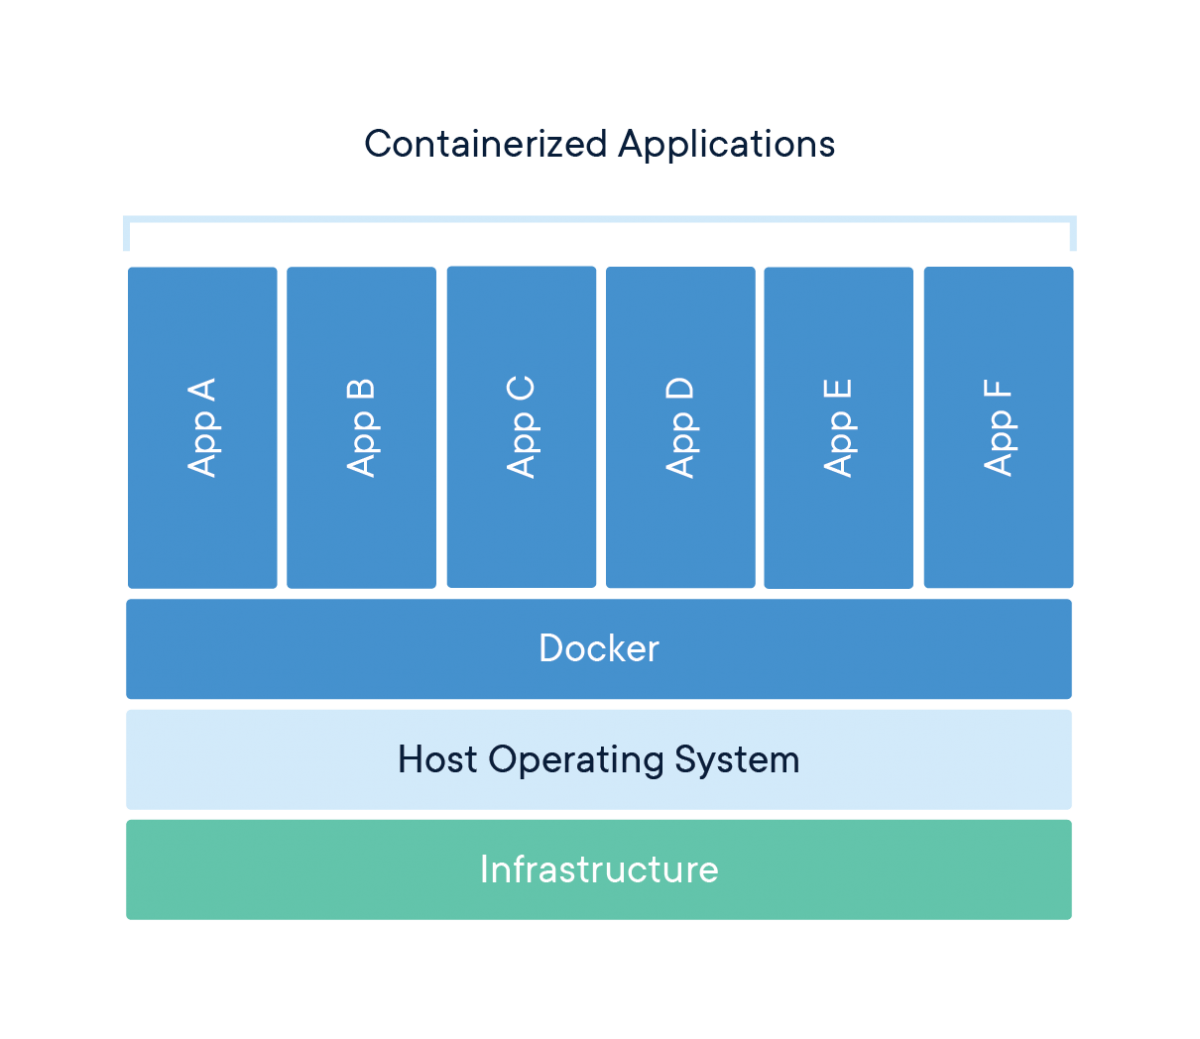
\includegraphics[ width = 10cm]{chapters/images/ch_2/Tools/container-what-is-container.png}
    \caption{Structure of containerized applications. \cite{container}}
    \label{fig:containers}
\end{figure}

\subsection{Kubernetes} %usiamo rancher come cluster k8s
In a production environment there is a need to manage containers running applications and ensure there is no downtime, and Kubernetes (K8s)\cite{k8s} provides a framework to run distributed systems in a resilient manner, by taking care of the scaling and failover, and providing deployment patterns.

Some of the features provided by Kubernetes are: 
\begin{itemize}
    \item \emph{Service discovery and load balancing}: exposing a container via a DNS name or IP address, and if the traffic to the container is high, it can create a new instance of the same container image and perform load balancing by distributing network traffic between them. This feature is widely used in the context of the project.
    \item \emph{Storage orchestration}: allows to automatically mount a chosen storage system, being it local, cloud hosted, or some other place.
    \item \emph{Automated rollouts and rollbacks}: gives the possibility of automatically deploy and remove containers, and move resources between them.
    \item \emph{Automatic bin packing}: once decided the amount of CPU and memory (RAM) needed by a container, it automatically place containers in node clusters to make the best use of the resources.
    \item \emph{Self-healing}: automatically restart failed containers, replaces them, and kills unresponsive ones.
    \item \emph{Secret and configuration management}: allows to store sensitive information that can be deployed or updated without the need to rebuild the container images.
\end{itemize}

\subsection*{Rancher}
The tool used for the orchestration of Kubernetes clusters is Rancher \cite{rancher}, an open source platform that makes it easy to create, manage, and monitor them.
\begin{definition}
Rancher is a software product to manage Kubernetes clusters. This includes not only managing existing clusters, but building new clusters as well. \cite{wRancher}
\end{definition}


